\documentclass[12pt]{article}

\usepackage{cmap} % Fixes search and copy-paste for Cyrillic in PDF
\usepackage[T2A]{fontenc}
\usepackage[utf8]{inputenc}
\usepackage[bulgarian]{babel}

% --- Typography ---
\usepackage{tempora} % Better Times New Roman clone with full Cyrillic support
\usepackage[top=2.5cm, bottom=2.5cm, left=3.0cm, right=2.0cm, a4paper]{geometry}
\usepackage{setspace}
\setstretch{1.5} % 1.5 line spacing
\usepackage[none]{hyphenat} % No hyphenation
\usepackage[expansion=false]{microtype} % Better text spacing and overflow prevention
\emergencystretch=1.5em % Help with line breaks in no-hyphenation environment
\sloppy
\usepackage{indentfirst} % Indent first paragraph after section
\setlength{\parindent}{1.25cm}
\setlength{\parskip}{0pt}

% --- Page Numbering (Bottom Right) ---
\usepackage{fancyhdr}
\pagestyle{fancy}
\fancyhf{}
\renewcommand{\headrulewidth}{0pt}
\fancyfoot[R]{\thepage}

% --- Footnotes ---
\usepackage[hang,flushmargin]{footmisc}
\usepackage{ragged2e}
\renewcommand{\footnotelayout}{\fontsize{10}{12}\selectfont\setstretch{1.0}\justifying}

% --- Section Formatting ---
\usepackage{titlesec}
\newcommand{\sectionbreak}{\clearpage}

% Numbering style
\renewcommand{\thesection}{\Roman{section}}
\renewcommand{\thesubsection}{\arabic{section}.\arabic{subsection}}
\renewcommand{\thesubsubsection}{\arabic{section}.\arabic{subsection}.\arabic{subsubsection}}

% Sections: Roman, Bold, 14pt, Centered, Uppercase
\titleformat{\section}[block]
  {\fontsize{14}{16.8}\bfseries\centering}
  {\thesection. }
  {0pt}
  {\MakeUppercase}

% Paragraphs: Arabic, Bold, 14pt, 1.25cm indent
\titleformat{\subsection}[block]
  {\fontsize{14}{16.8}\bfseries}
  {\thesubsection. }
  {0pt}
  {}
\titlespacing*{\subsection}{1.25cm}{*3}{*2}

% Sub-paragraphs: Bold, 13pt, 2.0cm indent
\titleformat{\subsubsection}[block]
  {\fontsize{13}{15.6}\bfseries}
  {\thesubsubsection. }
  {0pt}
  {}
\titlespacing*{\subsubsection}{2.0cm}{*2}{*1}

% TOC uppercase patches
\usepackage{etoolbox}
\makeatletter
\patchcmd{\l@section}{#1}{\MakeUppercase{#1}}{}{}
\makeatother
\usepackage[titles]{tocloft}
\renewcommand{\cftsecleader}{\cftdotfill{\cftdotsep}}
\renewcommand{\cftsubsecleader}{\cftdotfill{\cftdotsep}}
\renewcommand{\cftsubsubsecleader}{\cftdotfill{\cftdotsep}}
\renewcommand{\cftsecfont}{\fontsize{12}{14}\bfseries}
\renewcommand{\cftsecpagefont}{\fontsize{12}{14}\bfseries}
\renewcommand{\cftsecaftersnum}{.}
\renewcommand{\cftsubsecaftersnum}{.}
\renewcommand{\cftsubsubsecaftersnum}{.}

% --- Captions (Tables & Figures) ---
\usepackage{caption}
\DeclareCaptionLabelFormat{tablelabel}{Таблица #2}
\captionsetup[table]{
    labelformat=tablelabel, 
    labelsep=period, 
    font={bf,small}, % small is ~11pt in 12pt document
    justification=centering, 
    singlelinecheck=true
}
\DeclareCaptionLabelFormat{figurelabel}{Фигура #2}
\captionsetup[figure]{
    labelformat=figurelabel, 
    labelsep=period, 
    font={bf,small}, 
    justification=centering,
    singlelinecheck=true
}

% --- Other Essential Packages (Restored from original) ---
\usepackage{amsmath,amssymb,amsfonts}
\usepackage{amsthm}
\usepackage{graphicx}
\DeclareGraphicsExtensions{.tif,.png,.jpg,.pdf}
\usepackage{float}
\usepackage{booktabs}
\usepackage{longtable}
\usepackage{multirow}
\usepackage{hyperref}
\usepackage{listings}
\usepackage{xcolor}
\usepackage{tikz}
\usetikzlibrary{decorations.pathreplacing}
\usepackage{siunitx}
\usepackage{textcomp}
\usepackage{gensymb}
\usepackage{fancyvrb}
\usepackage{eurosym}
\usepackage{soul}
\usepackage{subcaption}
\usepackage{enumerate}
\usepackage{enumitem}
\usepackage{adjustbox}

% --- Single Spacing Fixes ---
% Reset to single spacing for common non-text environments
\AtBeginEnvironment{tikzpicture}{\setstretch{1.1}}
\AtBeginEnvironment{lstlisting}{\setstretch{1.1}}
\AtBeginEnvironment{verbatim}{\setstretch{1.1}}
\AtBeginEnvironment{tabular}{\setstretch{1.1}}
\AtBeginEnvironment{tabu}{\setstretch{1.1}}
\AtBeginEnvironment{longtable}{\setstretch{1.1}}

% Global TikZ overflow fix: wrap in adjustbox
\BeforeBeginEnvironment{tikzpicture}{\begin{adjustbox}{max width=\textwidth}}
\AfterEndEnvironment{tikzpicture}{\end{adjustbox}}

% --- Code Highlighting ---
\definecolor{cppblue}{RGB}{0,0,180}
\definecolor{cppgreen}{RGB}{0,128,0}
\definecolor{cppred}{RGB}{180,0,0}
\definecolor{cppgray}{RGB}{128,128,128}

% Use a slightly more compact font for code to prevent horizontal overflow
% \usepackage[scaled=0.85]{couriers} % Removed because it lacks Cyrillic support, leading to spacing issues in code blocks
\usepackage[T2A]{fontenc} % Ensure T2A is available for the default typewriter font
\lstset{
    language=C++,
    basicstyle=\small\ttfamily,
    breaklines=true,
    breakatwhitespace=true,
    columns=fullflexible, % Better width handling for mono fonts
    keepspaces=true,
    xleftmargin=1.5em,
    xrightmargin=0.5em,
    keywordstyle=\color{cppblue}\bfseries,
    stringstyle=\color{cppred},
    commentstyle=\color{cppgreen}, % Removed itshape as it often causes spacing issues with Cyrillic
    identifierstyle=\color{black},
    showstringspaces=false,
    numbers=left,
    numberstyle=\tiny\color{cppgray},
    numbersep=8pt,
    aboveskip=1.5em,
    belowskip=1.5em,
    frame=single,
    framerule=0.5pt,
    rulecolor=\color{cppgray},
    tabsize=4,
    captionpos=b,
    morekeywords={co_await, co_return, co_yield, Task, expected, unexpected, requires, concept, constexpr, noexcept, nullptr, override, final},
    emph={Request, Response, Handler, Middleware, Router, App, Connection, WebSocketConnection, IoContext},
    emphstyle=\color{cppblue},
    columns=fullflexible,
    inputencoding=utf8,
    literate={а}{{\cyra}}1 {б}{{\cyrb}}1 {в}{{\cyrv}}1 {г}{{\cyrg}}1 {д}{{\cyrd}}1
             {е}{{\cyre}}1 {ж}{{\cyrzh}}1 {з}{{\cyrz}}1 {и}{{\cyri}}1 {й}{{\cyrishrt}}1
             {к}{{\cyrk}}1 {л}{{\cyrl}}1 {м}{{\cyrm}}1 {н}{{\cyrn}}1 {о}{{\cyro}}1
             {п}{{\cyrp}}1 {р}{{\cyrr}}1 {с}{{\cyrs}}1 {т}{{\cyrt}}1 {у}{{\cyru}}1
             {ф}{{\cyrf}}1 {х}{{\cyrh}}1 {ц}{{\cyrc}}1 {ч}{{\cyrch}}1 {ш}{{\cyrsh}}1
             {щ}{{\cyrshch}}1 {ъ}{{\cyrhrdsn}}1 {ь}{{\cyrsftsn}}1 {ю}{{\cyryu}}1 {я}{{\cyrya}}1
             {А}{{\CYRA}}1 {Б}{{\CYRB}}1 {В}{{\CYRV}}1 {Г}{{\CYRG}}1 {Д}{{\CYRD}}1
             {Е}{{\CYRE}}1 {Ж}{{\CYRZH}}1 {З}{{\CYRZ}}1 {И}{{\CYRI}}1 {Й}{{\CYRISHRT}}1
             {К}{{\CYRK}}1 {Л}{{\CYRL}}1 {М}{{\CYRM}}1 {Н}{{\CYRN}}1 {О}{{\CYRO}}1
             {П}{{\CYRP}}1 {Р}{{\CYRR}}1 {С}{{\CYRS}}1 {Т}{{\CYRT}}1 {У}{{\CYRU}}1
             {Ф}{{\CYRF}}1 {Х}{{\CYRH}}1 {Ц}{{\CYRC}}1 {Ч}{{\CYRCH}}1 {Ш}{{\CYRSH}}1
             {Щ}{{\CYRSHCH}}1 {Ъ}{{\CYRHRDSN}}1 {Ь}{{\CYRSFTSN}}1 {Ю}{{\CYRYU}}1 {Я}{{\CYRYA}}1,
}

\begin{document}

% --- Title Page ---
\begin{titlepage}
\begin{center}
    {\fontsize{18}{21.6}\selectfont\bfseries ТЕХНИЧЕСКИ УНИВЕРСИТЕТ – СОФИЯ\par}
    \vspace{0.5cm}
    {\fontsize{16}{19.2}\selectfont\bfseries ФАКУЛТЕТ „КОМПЮТЪРНИ СИСТЕМИ И ТЕХНОЛОГИИ”\par}
    
    \vspace{0.5cm}
    \begin{figure}[H]
        \centering
        
\includegraphics[width=0.4\linewidth]{images/ту.png}
    \end{figure}
    \vspace{0.5cm}
    
    {\fontsize{20}{24}\selectfont\bfseries Лабораторно упражнение №: 3\par Мащабиране на изображения и анализ на пространствени артефакти\par}
    
    \vspace{1.5cm}
    
    {\fontsize{14}{16.8}\selectfont\bfseries Цифрова обработка на изображения\par}
    
    \vfill
    
    \begin{flushleft}
    {\fontsize{14}{16.8}\selectfont\bfseries Изготвил:\par}
    Кирил Вълков, фак. № 121222194\par
    Специалност: Компютърно и софтуерно инженерство\par
    
    \vspace{1cm}
    
    {\fontsize{14}{16.8}\selectfont\bfseries Научен ръководител:\par}
    доц. д-р инж. Ива Николова\par
    \end{flushleft}
    
    \vfill
    
    {\fontsize{12}{14.4}\selectfont София, \today \par}
\end{center}
\end{titlepage}

\newpage
\pagenumbering{roman}
\tableofcontents
\newpage

\pagenumbering{arabic}
\section{ЕКСПЕРИМЕНТАЛНИ РЕЗУЛТАТИ}
\section{ЦЕЛ НА УПРАЖНЕНИЕТО}
Целта на упражнението е да се изследват процесите на мащабиране (намаляване и увеличаване) на цифрови изображения и възникващите пространствени артефакти, като aliasing и блоков ефект. Разглежда се ролята на предварителната нискочестотна филтрация (anti-aliasing) за подобряване на качеството при децимация. Резултатите се оценяват както визуално, така и количествено чрез метриките MSE и PSNR.

\section{РЕЗУЛТАТИ И АНАЛИЗ ПО ЗАДАНИЯ}

\subsection{Задание 1 – Намаляване на изображение чрез избор на пиксели}
\subsubsection{Резултати}

\textbf{Реализация на функциите за намаляване:}
\begin{lstlisting}[language=Matlab]
% ds_factor2_A.m
function I_out = ds_factor2_A(I_in)
    [M,N] = size(I_in);
    I_out = I_in(1:2:2*floor(M/2), 1:2:2*floor(N/2));
endfunction

% ds_factor2_B.m
function I_out = ds_factor2_B(I_in)
    [M,N] = size(I_in);
    M4 = floor(M/4)*4;
    N4 = floor(N/4)*4;
    I_in = I_in(1:M4,1:N4);
    I_out = zeros(M4/2, N4/2);
    for r = 1:4:M4
        for c = 1:4:N4
            r_out = floor(r/2) + 1;
            c_out = floor(c/2) + 1;
            I_out(r_out:r_out+1, c_out:c_out+1) = I_in(r:r+1, c:c+1);
        end
    end
endfunction
\end{lstlisting}

% checkerboard_test.png
\begin{figure}[H]
\centering
\begin{subfigure}[b]{0.3\textwidth}

\includegraphics[width=\textwidth]{../results/task1_original_checkerboard_test.png}
\caption{Оригинал (checkerboard)}
\end{subfigure}
\hfill
\begin{subfigure}[b]{0.3\textwidth}

\includegraphics[width=\textwidth]{../results/task1_A_checkerboard_test.png}
\caption{Схема A}
\end{subfigure}
\hfill
\begin{subfigure}[b]{0.3\textwidth}

\includegraphics[width=\textwidth]{../results/task1_B_checkerboard_test.png}
\caption{Схема B}
\end{subfigure}

\vspace{0.3cm}
\begin{subfigure}[b]{0.3\textwidth}
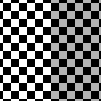
\includegraphics[width=\textwidth]{../results/task1_zoom_original_checkerboard_test.png}
\caption{Оригинал (Zoom)}
\end{subfigure}
\hfill
\begin{subfigure}[b]{0.3\textwidth}
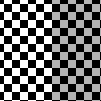
\includegraphics[width=\textwidth]{../results/task1_zoom_A_checkerboard_test.png}
\caption{Схема A (Zoom)}
\end{subfigure}
\hfill
\begin{subfigure}[b]{0.3\textwidth}
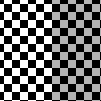
\includegraphics[width=\textwidth]{../results/task1_zoom_B_checkerboard_test.png}
\caption{Схема B (Zoom)}
\end{subfigure}
\caption{Резултати от децимация: checkerboard\_test.png}
\end{figure}

% siemens_star.png
\begin{figure}[H]
\centering
\begin{subfigure}[b]{0.3\textwidth}
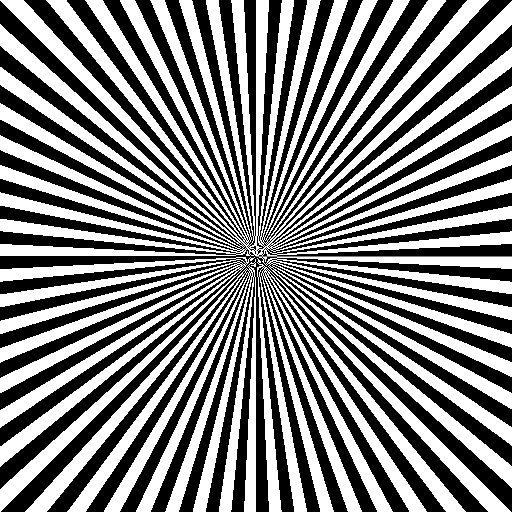
\includegraphics[width=\textwidth]{../results/task1_original_siemens_star.png}
\caption{Оригинал (siemens\_star)}
\end{subfigure}
\hfill
\begin{subfigure}[b]{0.3\textwidth}

\includegraphics[width=\textwidth]{../results/task1_A_siemens_star.png}
\caption{Схема A}
\end{subfigure}
\hfill
\begin{subfigure}[b]{0.3\textwidth}
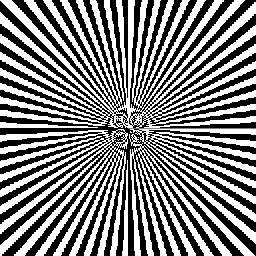
\includegraphics[width=\textwidth]{../results/task1_B_siemens_star.png}
\caption{Схема B}
\end{subfigure}

\vspace{0.3cm}
\begin{subfigure}[b]{0.3\textwidth}
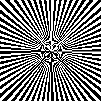
\includegraphics[width=\textwidth]{../results/task1_zoom_original_siemens_star.png}
\caption{Оригинал (Zoom)}
\end{subfigure}
\hfill
\begin{subfigure}[b]{0.3\textwidth}
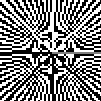
\includegraphics[width=\textwidth]{../results/task1_zoom_A_siemens_star.png}
\caption{Схема A (Zoom)}
\end{subfigure}
\hfill
\begin{subfigure}[b]{0.3\textwidth}
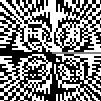
\includegraphics[width=\textwidth]{../results/task1_zoom_B_siemens_star.png}
\caption{Схема B (Zoom)}
\end{subfigure}
\caption{Резултати от децимация: siemens\_star.png}
\end{figure}

% kodim13.png
\begin{figure}[H]
\centering
\begin{subfigure}[b]{0.3\textwidth}

\includegraphics[width=\textwidth]{../results/task1_original_kodim13.png}
\caption{Оригинал (kodim13)}
\end{subfigure}
\hfill
\begin{subfigure}[b]{0.3\textwidth}

\includegraphics[width=\textwidth]{../results/task1_A_kodim13.png}
\caption{Схема A}
\end{subfigure}
\hfill
\begin{subfigure}[b]{0.3\textwidth}

\includegraphics[width=\textwidth]{../results/task1_B_kodim13.png}
\caption{Схема B}
\end{subfigure}

\vspace{0.3cm}
\begin{subfigure}[b]{0.3\textwidth}

\includegraphics[width=\textwidth]{../results/task1_zoom_original_kodim13.png}
\caption{Оригинал (Zoom)}
\end{subfigure}
\hfill
\begin{subfigure}[b]{0.3\textwidth}

\includegraphics[width=\textwidth]{../results/task1_zoom_A_kodim13.png}
\caption{Схема A (Zoom)}
\end{subfigure}
\hfill
\begin{subfigure}[b]{0.3\textwidth}

\includegraphics[width=\textwidth]{../results/task1_zoom_B_kodim13.png}
\caption{Схема B (Zoom)}
\end{subfigure}
\caption{Резултати от децимация: kodim13.png}
\end{figure}

% Img08.tif
\begin{figure}[H]
\centering
\begin{subfigure}[b]{0.3\textwidth}

\includegraphics[width=\textwidth]{../results/task1_original_Img08.png}
\caption{Оригинал (Img08)}
\end{subfigure}
\hfill
\begin{subfigure}[b]{0.3\textwidth}

\includegraphics[width=\textwidth]{../results/task1_A_Img08.png}
\caption{Схема A}
\end{subfigure}
\hfill
\begin{subfigure}[b]{0.3\textwidth}

\includegraphics[width=\textwidth]{../results/task1_B_Img08.png}
\caption{Схема B}
\end{subfigure}

\vspace{0.3cm}
\begin{subfigure}[b]{0.3\textwidth}

\includegraphics[width=\textwidth]{../results/task1_zoom_original_Img08.png}
\caption{Оригинал (Zoom)}
\end{subfigure}
\hfill
\begin{subfigure}[b]{0.3\textwidth}

\includegraphics[width=\textwidth]{../results/task1_zoom_A_Img08.png}
\caption{Схема A (Zoom)}
\end{subfigure}
\hfill
\begin{subfigure}[b]{0.3\textwidth}

\includegraphics[width=\textwidth]{../results/task1_zoom_B_Img08.png}
\caption{Схема B (Zoom)}
\end{subfigure}
\caption{Резултати от децимация: Img08.tif}
\end{figure}

\subsubsection{Анализ}
\begin{itemize}
    \item \textbf{Наблюдавани артефакти:} Различните изображения ясно показват ефекта на припокриване (aliasing) при децимация чрез Схема А: \textbf{checkerboard} губи строгата си периодична структура; \textbf{siemens\_star} проявява силни муарови (Moiré) шарки в центъра си, където пространствената честота е най-голяма; при \textbf{kodim13} и \textbf{Img08} се наблюдават назъбени ръбове (jaggies) в детайлните участъци. При Схема В (копиране на 2x2 блокове със стъпка 4), освен наличието на aliasing, се получава и силен блоков ефект, като изображението става грубо накъсано (най-вече при сименсовата звезда).
    \item \textbf{Локализация на изкривяванията:} Най-явните изкривявания се наблюдават в центъра на сименсовата звезда, в пресечните точки на checkerboard и по тънките линии, мрежи, козина и остри ръбове в реалните изображения.
    \item \textbf{Причини за aliasing:} Aliasing възниква, когато честотата на дискретизация (в случая, пространственото разреждане на пикселите при намаляване) е по-малка от удвоената максимална честота в изображението (нарушаване на теоремата на Найкуист-Шанън). Високите честоти погрешно се интерпретират като ниски, създавайки фалшиви модели (муарови шарки).
    \item \textbf{Визуална разлика между Схема A и B:} Схема А запазва общата структура по-рязка, но с по-забележимо трептене и муар на фините детайли. Схема B изглежда цялостно по-размазана и груба (поради съседните дублирани пиксели), блокирайки някои от най-фините детайли.
\end{itemize}

\subsection{Задание 2 – Нискочестотна филтрация и количествен анализ}
\subsubsection{Резултати}

\begin{figure}[H]
\centering
\begin{subfigure}[b]{0.3\textwidth}

\includegraphics[width=\textwidth]{../results/task2_Ir.png}
\caption{Референтно ($I_r$)}
\end{subfigure}
\hfill
\begin{subfigure}[b]{0.3\textwidth}

\includegraphics[width=\textwidth]{../results/task2_FA.png}
\caption{Схема F+A}
\end{subfigure}
\hfill
\begin{subfigure}[b]{0.3\textwidth}

\includegraphics[width=\textwidth]{../results/task2_FB.png}
\caption{Схема F+B}
\end{subfigure}
\caption{Резултати след предварителна нискочестотна филтрация}
\end{figure}

\begin{figure}[H]
\centering
\begin{subfigure}[b]{0.3\textwidth}

\includegraphics[width=\textwidth]{../results/task2_zoom_Ir.png}
\caption{Референтно (Zoom)}
\end{subfigure}
\hfill
\begin{subfigure}[b]{0.3\textwidth}

\includegraphics[width=\textwidth]{../results/task2_zoom_FA.png}
\caption{Схема F+A (Zoom)}
\end{subfigure}
\hfill
\begin{subfigure}[b]{0.3\textwidth}

\includegraphics[width=\textwidth]{../results/task2_zoom_FB.png}
\caption{Схема F+B (Zoom)}
\end{subfigure}
\caption{Приближение на филтрираните изображения в сравнение с референтното}
\end{figure}

\begin{table}[H]
\centering
\begin{tabular}{|c|c|c|}
\hline
\textbf{Вариант} & \textbf{MSE} & \textbf{PSNR (dB)} \\
\hline
A & 0.003870 & 24.12 \\
\hline
B & 0.006699 & 21.74 \\
\hline
F+A & 0.000766 & 31.16 \\
\hline
F+B & 0.002221 & 26.53 \\
\hline
\end{tabular}
\caption{Количествена оценка на методите за намаляване спрямо референтно изображение $I_r$}
\end{table}

\subsubsection{Анализ}
\begin{itemize}
    \item \textbf{Сравнение на MSE и PSNR:} Филтрираните варианти (F+A и F+B) показват значително по-нисък MSE и съответно по-висок PSNR. Това потвърждава, че предварителната нискочестотна филтрация намалява грешката при мащабиране надолу. Схема F+A е с най-висок PSNR (31.16 dB) и видимо се доближава най-много до бикубичната интерполация ($I_r$).
    \item \textbf{Роля на предварителната филтрация:} Нискочестотният филтър премахва високочестотните компоненти, които биха причинили aliasing при децимацията. Той служи като anti-aliasing филтър, осигурявайки по-плавно пренасяне на границите.
    \item \textbf{Визуално подобрение:} Подобрението е най-явно в зони с фини повтарящи се текстури. Козината и тънките линии изглеждат значително по-меки и стабилни, без назъбени фалшиви структурни мотиви (муар).
    \item \textbf{Количествена vs. Визуална оценка:} Визуалната оценка напълно се припокрива с метриките: F+A безспорно изглежда по-приятно от чисто А, и това е отчетено със скок на PSNR от 24.12 на 31.16 dB.
\end{itemize}

\subsection{Задание 3 – Увеличаване чрез интерполация „най-близък съсед“}
\subsubsection{Резултати}

\textbf{Реализация на функцията за увеличаване:}
\begin{lstlisting}[language=Matlab]
% upsample_nn_x2.m
function I_out = upsample_nn_x2(I_in)
    [M, N] = size(I_in);
    I_out = zeros(2*M, 2*N);
    for r = 1:M
        for c = 1:N
            I_out(2*r-1:2*r, 2*c-1:2*c) = I_in(r, c);
        end
    end
endfunction
\end{lstlisting}

\begin{figure}[H]
\centering
\begin{subfigure}[b]{0.45\textwidth}

\includegraphics[width=\textwidth]{../results/task3_A.png}
\caption{А $\rightarrow$ NN}
\end{subfigure}
\hfill
\begin{subfigure}[b]{0.45\textwidth}

\includegraphics[width=\textwidth]{../results/task3_B.png}
\caption{B $\rightarrow$ NN}
\end{subfigure}
\begin{subfigure}[b]{0.45\textwidth}

\includegraphics[width=\textwidth]{../results/task3_FA.png}
\caption{F+A $\rightarrow$ NN}
\end{subfigure}
\hfill
\begin{subfigure}[b]{0.45\textwidth}

\includegraphics[width=\textwidth]{../results/task3_FB.png}
\caption{F+B $\rightarrow$ NN}
\end{subfigure}
\caption{Увеличаване (x2) чрез „най-близък съсед“ (NN)}
\end{figure}

\begin{figure}[H]
\centering
\begin{subfigure}[b]{0.3\textwidth}

\includegraphics[width=\textwidth]{../results/task3_zoom_A.png}
\caption{A $\rightarrow$ NN (Zoom)}
\end{subfigure}
\hfill
\begin{subfigure}[b]{0.3\textwidth}

\includegraphics[width=\textwidth]{../results/task3_zoom_B.png}
\caption{B $\rightarrow$ NN (Zoom)}
\end{subfigure} % add spacing issue fix below
\vspace{0.3cm}
\begin{subfigure}[b]{0.3\textwidth}

\includegraphics[width=\textwidth]{../results/task3_zoom_FA.png}
\caption{F+A $\rightarrow$ NN (Zoom)}
\end{subfigure}
\hfill
\begin{subfigure}[b]{0.3\textwidth}

\includegraphics[width=\textwidth]{../results/task3_zoom_FB.png}
\caption{F+B $\rightarrow$ NN (Zoom)}
\end{subfigure}
\caption{Приближение (zoom-in) на възстановените изображения}
\end{figure}


\begin{table}[H]
\centering
\begin{tabular}{|c|c|c|}
\hline
\textbf{Вариант} & \textbf{MSE} & \textbf{PSNR (dB)} \\
\hline
А $\rightarrow$ NN & 0.007257 & 21.39 \\
\hline
B $\rightarrow$ NN & 0.011024 & 19.58 \\
\hline
F+A $\rightarrow$ NN & 0.004805 & 23.18 \\
\hline
F+B $\rightarrow$ NN & 0.006382 & 21.95 \\
\hline
\end{tabular}
\caption{Количествена оценка на методите за увеличаване спрямо оригиналното изображение}
\end{table}

\subsubsection{Анализ}
\begin{itemize}
    \item \textbf{Артефакти при Nearest Neighbor (NN):} Основният артефакт е "блоковият ефект" (pixelation). Тъй като интерфейсът просто копира стойностите на пикселите, диагоналните линии и кривите придобиват силно начупен, стъпаловиден вид.
    \item \textbf{Сравнение с филтрация и без:} Филтрираните варианти изглеждат по-размазани в резултат на нискочестотната обработка, но значително ограничават назъбването спрямо нефилтрираните. Високите честоти, които пораждат алиасинг в първичната стъпка (схема A/B), вече липсват.
    \item \textbf{Влияние на намаляването спрямо увеличаването:} Намаляването (и съответната загуба на информация) оказва по-осезаемо фундаментално влияние, тъй като веднъж щом високите честоти бъдат премахнати или изкривени (aliasing), те не могат да бъдат възстановени. Увеличаването чрез NN по-скоро влошава визуално нещата с допълнителни блокови артефакти, но основната структурна щета е направена при намаляването.
    \item \textbf{Възстановяване на детайли:} Интерполацията "най-близък съсед" \textbf{не може} да възстанови изгубените високочестотни детайли. Тя работи локално само с наличната вече оскъдна информация и генерира фалшиви високи честоти чрез остри преходи между дублираните блокове (пикселизация).
\end{itemize}

\section{ОБЩИ ИЗВОДИ}

\begin{itemize}
    \item \textbf{Влияние на мащабирането:} Намаляването без филтрация перманентно унищожава високочестотна информация и предизвиква силен алиасинг при честоти над хипотетичната граница на Найкуист. Увеличаването чрез NN е най-елементарната техника, която подчертава ниското разрешение чрез блокови ефекти. На този етап по-сложна интерполация (като бикубична) би била за предпочитане за по-гладки резултати.
    \item \textbf{Роля на нискочестотната филтрация:} Приложението на Gauss филтър преди децимация е жизнено важно. Макар че жертва абсолютната острота, филтърът действа като anti-aliasing механизъм и произвежда в пъти по-натурално и леко за възприемане изображение с драстичен скок в PSNR (от 24 dB на над 31 dB).
    \item \textbf{Метрики vs. възприятие:} MSE и PSNR са добри индикатори за структурна близост, като се наблюдават консистентни с човешкото зрение резултати (напр. филтрираната A схема е обективно изчислена като най-високо качество). В някои гранични случаи обаче, PSNR може да фаворизира "прекалено замазано" изображение пред по-остро, но леко пикселизирано, поради спецификата на квадратичната еквализация при MSE.
\end{itemize}

\end{document}

